\documentclass{article}
\usepackage[utf8]{inputenc}
\usepackage[a4paper, margin=1in]{geometry}
\usepackage{graphicx}
\usepackage{natbib}
\bibliographystyle{apalike}

\title{Visualizing the Decline in Cultural Participation in Europe Post-Crisis}
\author{Omar Lizardo}
\date{February 2023}

\begin{document}

\maketitle

\section{Introduction}

\section{The decline in cultural participation post-crisis}

Figure~\ref{fig: main} shows stacked bar plots designed for the analysis and presentation of Likert-type data \citep{heiberger2014design}, rendered using the {\em} R-package \texttt{likert} created by Jason Bryer \citeyearpar{bryer-likert}. In the figure each horizontal bar represents the number of six possible cultural activities undertaken by respondents in the previous year in four ordered categories: None, one to two, three to four, and five to six. The activities include (1) Going to the movies, (2) Attending a dance performance, (3) Attending a museum or a gallery, (4) Attending a musical concert, (5) Visiting a historical monument, and (6) attending a dramatic or theater performance. 

Looking at panels (a) and (b) we can see that three out of the four Southern European countries, with the possible exception of Spain, experienced steep increases in cultural non-participation post-crisis. The proportion of people who report doing none of the cultural activities goes from 46\%, 31\%, 43\%, and 25\% in 2007 for Portugal, Spain, Greece and Italy, to 59\%, 36\%, 52\%, and 34\%, respectively. 

Is there heterogeneity in the decline in cultural participation across respondents with different levels of education? We know from previous work that education is the best predictor of cultural participation, and that the cultural participation habit of the more educated are more resistant to exogenous shocks. Moreover, education is correlated with earnings, which means that any restrictions on leisure consumption for cultural goods should hit the less educated the hardest. 

Looking at panels c-d, we find that the decline in cultural participation affected people with more and less education differently in each national case, although overall, the expectation that the crisis affected does with less education seems to hold. First, note that steep cultural capital gradient on cultural participation. Across all national cases and periods, the more educated are more likely to participate in cultural activities.  

Looking at specific combinations of country and period, we see that in Portugal (panels c-d), the increase in non-participation is concentrated among people with about a high-school education (16–19 years old when they completed schooling), who went from a non-participation rate of 22\% in 2007 to 40\% in 2013. Respondent's with a university education were relatively protected (14\% versus 16\%); in fact, for this group the proportion engaging in the most activities (five to six) seems to have grown post-crisis. In Spain (panels e-f), we find the same pattern, although with a less steep increase in non-participation going from 17\% to 25\% among the high-school educated. Italy tells the same story, although there we also observe relatively big increases in non-participation for those with less than a high-school education, who go from 47\% with zero cultural activities in 2007 to 58\% in 2013. Finally, Greece shows a different pattern from the three other Southern European cases, evincing a general increase in non-participation across {\em all} levels of education excepting stud

\begin{figure}
    \centering
    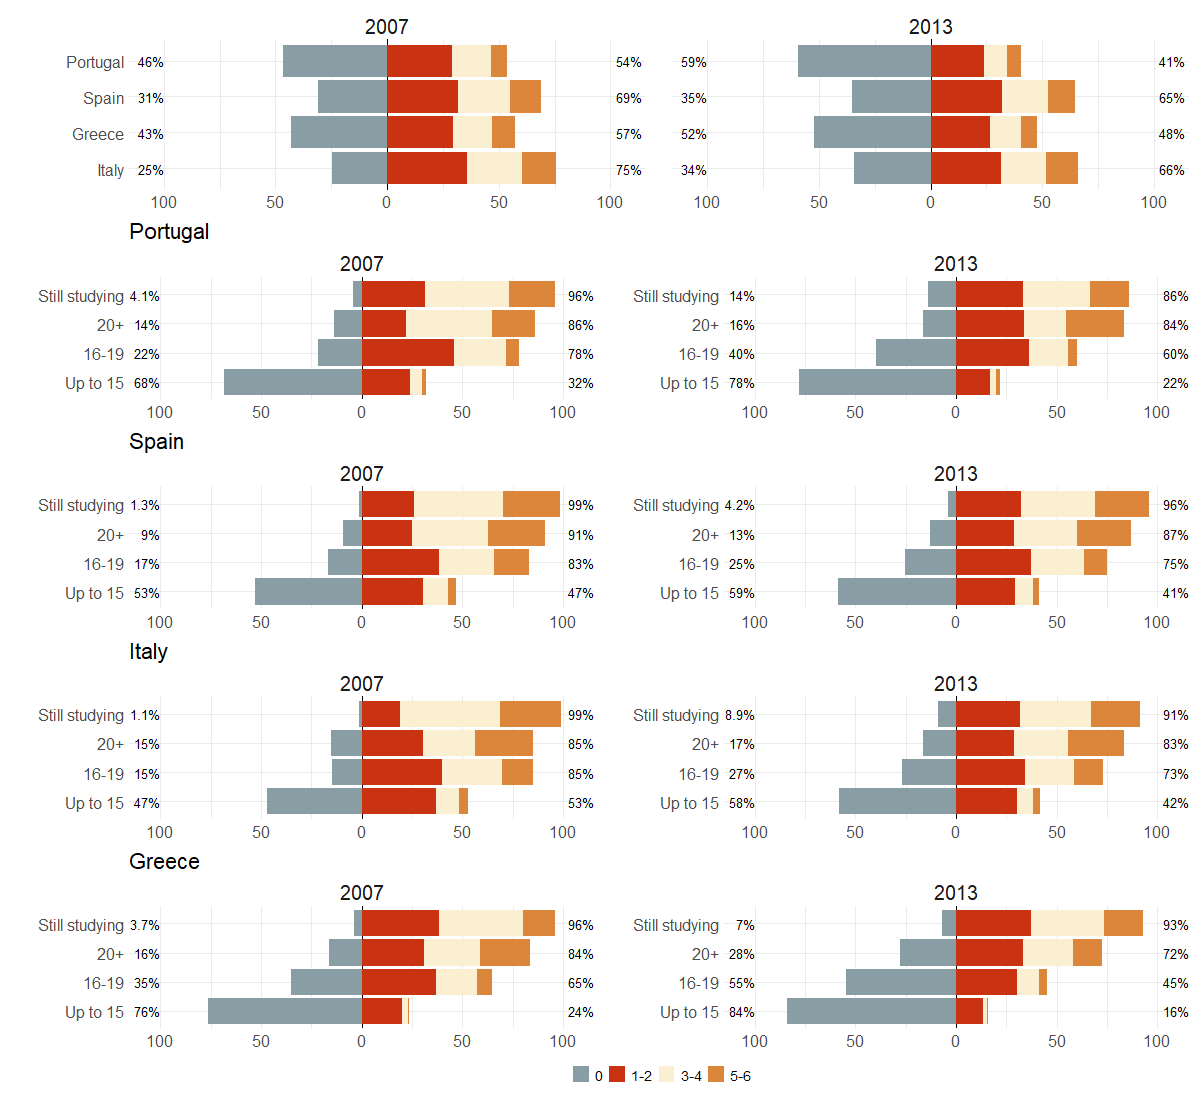
\includegraphics[width=1.0\textwidth]{Plots/cult-cat2-by-year-by-country-combo.png}
    \caption{Stacked bar plots of number of cultural activities for four Southern European countries. the top panel (a-b) shows the number of cultural activities per country for 2007 (a) and 2013 (b). The bottom panels (c-j) show the number of cultural activities for each country in each year by the respondent's level of education; Portugal (c-d), Spain (e-f), Italy (g-h) and Greece (i-j). The color palette used in the plot is "Royal2" from Karthik Ram's \citeyearpar{Ram_wespalette} \texttt{wesanderson} {\em R} package.}
    \label{fig: main}
\end{figure}

\bibliography{main}
\end{document}
